\documentclass[
../../AuD-Zusammenfassung.tex,
]
{subfiles}

\externaldocument[ext:]{../../AuD-Zusammenfassung}
% Set Graphics Path, so pictures load correctly
\graphicspath{{../../}}

\begin{document}
\section{Graphen Algorithmen}
\subsection{Graphen}
Der abstrakter Datentyp der Graphen besteht im Grunde aus verschiedenen Knoten (vertices V), die Kanten (edges E) zu anderen Knoten haben. Sogesehen sind auch Bäume immer Graphen, wenn auch beschränkter.
\subsubsection{Gerichtete Graphen}
Gerichtete Graphen sind Graphen bei denen die edges E immer nur in eine Richtung sind. D.h., dass eine Kante von Knoten u nach Knoten v \textbf{nicht} gleichzusetzen ist wie eine Kante von Knoten v nach Knoten u. \\
In normaler Notation werden Kanten im Schema $(u,v)\in E$ angegeben, was eine Kante von Knoten u nach Knoten v darstellt.

\begin{minipage}[t]{\textwidth}
    \centering
    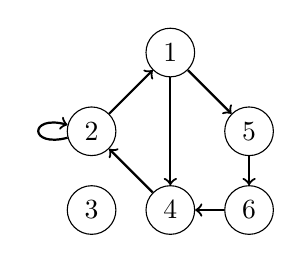
\begin{tikzpicture}[
        every node/.style={draw, minimum size=15pt, circle, text centered},
        ar/.style={->, thick},
        node distance = 22pt,
        invis/.style={draw=none},
    ]

    \node[](1) at (0,1) {1};
    \node[](4) at (0,-1) {4};
    \node[](2) at (-1,0) {2};
    \node[](5) at (1,0) {5};
    \node[](3) at (-1,-1) {3};
    \node[](6) at (1,-1) {6};

    \path[ar] 
    (1) edge (5) edge (4)
    (2) edge (1)

    (4) edge (2)
    (5) edge (6)
    (6) edge (4)
    ;
    \draw[ar, loop left] (2) to (2);
    \end{tikzpicture}
    \captionof*{figure}{Example}
    $V = \{1,2,3,4,5,6\}$\\
    $E = \{(1,4),(1,5),(2,1),(2,2),(4,2),(5,6),(6,4)\}$\\
    (3 hat keine Kanten weg oder zu sich, ist aber trotzdem Teil des Graphs)
\end{minipage}
\subsubsection{Ungerichtete Graphen}
Ungerichtete Graphen unterscheiden sich von gerichteten Graphen nur in der Hinsicht, dass die Kanten $(u,v)\in E$ und $(v,u) \in E$ gleichzusetzen sind.\\
\begin{minipage}[t]{\textwidth}
    \centering
    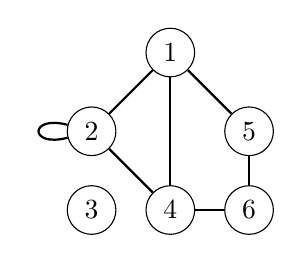
\begin{tikzpicture}[
        every node/.style={draw, minimum size=15pt, circle, text centered},
        ar/.style={-, thick},
        node distance = 22pt,
        invis/.style={draw=none},
    ]

    \node[](1) at (0,1) {1};
    \node[](4) at (0,-1) {4};
    \node[](2) at (-1,0) {2};
    \node[](5) at (1,0) {5};
    \node[](3) at (-1,-1) {3};
    \node[](6) at (1,-1) {6};

    \path[ar] 
    (1) edge (5) edge (4)
    (2) edge (1)

    (4) edge (2)
    (5) edge (6)
    (6) edge (4)
    ;
    \draw[ar, loop left] (2) to (2);
    \end{tikzpicture}
    \captionof*{figure}{Example}
    $V = \{1,2,3,4,5,6\}$\\
    $E = \{\{1,4\},\{1,5\},\{1,2\},\{2,2\}\{2,4\},\{4,6\},\{5,6\}\}$\\
    (Geschweifte Klammern stellen ungerichtete Kante dar)
\end{minipage}
\subsubsection{Pfade}
Ein Knoten $v$ ist von einem Knoten $u$ dann erreichbar, wenn es einen Pfad $(w_1,w_2,\ldots,w_k) \in V^k$ für den $(w_i,w_{i+1}) \in E$ für $i = 1,2,\ldots,k - 1$ und $w_1 = u$ und $w_k = v$ gibt.\\
(Ein Knoten ist immer von sich selbst erreichbar (leerer Pfad $k = 1$))\\
Dabei ist die Länge des Pfades mit $k - 1 =$ Anzahl der Kanten gegeben. $shortest(u,v) =$ Länge des kürzesten Pfades von $u$ nach $v$. 
\newpage
\subsubsection{Gewichtete Graphen}
Gewichtete Graphen haben zusätzlich bei den Kanten ein Gewicht. Dieses kann unterschiedliche Dinge, je nach Kontext bedeuten, bspw. könnte ein gewichteter Graph dazu genutzt werden Zugverbindungen darzustellen, wo die Knoten Haltestellen, die Kanten Zugverbindungen und die Gewichte die Entfernung darstellen. \\
Die Notation hierzu ist $w((u,v))$. Für ungerichtete gewichtete Graphen ist $w((u,v)) = w((v,u))$\\
\begin{minipage}[t]{\textwidth}
    \centering
    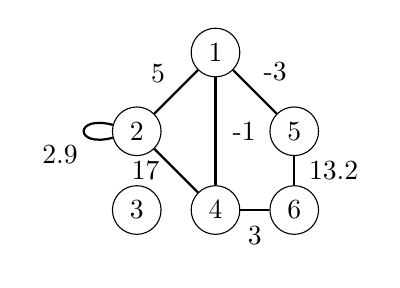
\begin{tikzpicture}[
        every node/.style={draw, minimum size=15pt, circle, text centered},
        ar/.style={-, thick},
        node distance = 22pt,
        invis/.style={draw=none},
    ]

    \node[](1) at (0,1) {1};
    \node[](4) at (0,-1) {4};
    \node[](2) at (-1,0) {2};
    \node[](5) at (1,0) {5};
    \node[](3) at (-1,-1) {3};
    \node[](6) at (1,-1) {6};

    \draw[ar] (1) to node[midway, above right, invis]{-3} (5);
    \draw[ar] (1) to node[midway, right, invis]{-1} (4);
    \draw[ar] (1) to node[midway, above left, invis]{5} (2);
    \draw[ar, loop left] (2) to node[midway, below left, invis]{2.9} (2);
    \draw[ar] (2) to node[midway, left, invis]{17} (4);
    \draw[ar] (4) to node[midway, below, invis]{3} (6);
    \draw[ar] (5) to node[midway, right, invis]{13.2} (6);


    \end{tikzpicture}
    \captionof*{figure}{Example}
\end{minipage}
\subsubsection{Zusammenhänge}
Ungerichtete Graphen gelten als \textbf{zusammenhängend}, wenn jeder Knoten von jedem anderen Knoten erreichbar ist. \\
\begin{minipage}[t]{0.5\textwidth}
    \centering
    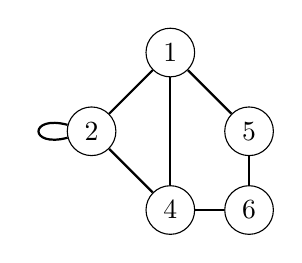
\begin{tikzpicture}[
        every node/.style={draw, minimum size=15pt, circle, text centered},
        ar/.style={-, thick},
        node distance = 22pt,
        invis/.style={draw=none},
    ]

    \node[](1) at (0,1) {1};
    \node[](4) at (0,-1) {4};
    \node[](2) at (-1,0) {2};
    \node[](5) at (1,0) {5};
    \node[](6) at (1,-1) {6};

    \path[ar] 
    (1) edge (5) edge (4)
    (2) edge (1)

    (4) edge (2)
    (5) edge (6)
    (6) edge (4)
    ;
    \draw[ar, loop left] (2) to (2);
    \end{tikzpicture}
    \captionof*{figure}{Zusammenhängend}
\end{minipage}
\begin{minipage}[t]{0.5\textwidth}
    \centering
    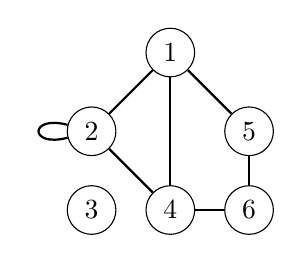
\begin{tikzpicture}[
        every node/.style={draw, minimum size=15pt, circle, text centered},
        ar/.style={-, thick},
        node distance = 22pt,
        invis/.style={draw=none},
    ]

    \node[](1) at (0,1) {1};
    \node[](4) at (0,-1) {4};
    \node[](2) at (-1,0) {2};
    \node[](5) at (1,0) {5};
    \node[](3) at (-1,-1) {3};
    \node[](6) at (1,-1) {6};

    \path[ar] 
    (1) edge (5) edge (4)
    (2) edge (1)

    (4) edge (2)
    (5) edge (6)
    (6) edge (4)
    ;
    \draw[ar, loop left] (2) to (2);
    \end{tikzpicture}
    \captionof*{figure}{Nicht zusammenhängend}
\end{minipage}
Ein gerichteter Graph gilt als \textbf{stark zusammenhängend}, wenn jeder Knoten von jedem anderen Knoten (beachte Kantenrichtung) erreichbar ist.\\
\begin{minipage}[t]{0.5\textwidth}
    \centering
    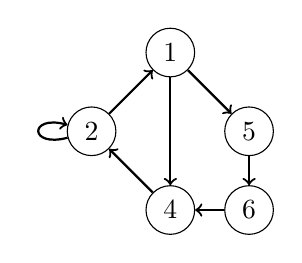
\begin{tikzpicture}[
        every node/.style={draw, minimum size=15pt, circle, text centered},
        ar/.style={->, thick},
        node distance = 22pt,
        invis/.style={draw=none},
    ]

    \node[](1) at (0,1) {1};
    \node[](4) at (0,-1) {4};
    \node[](2) at (-1,0) {2};
    \node[](5) at (1,0) {5};
    \node[](6) at (1,-1) {6};

    \path[ar] 
    (1) edge (5) edge (4)
    (2) edge (1)

    (4) edge (2)
    (5) edge (6)
    (6) edge (4)
    ;
    \draw[ar, loop left] (2) to (2);
    \end{tikzpicture}
    \captionof*{figure}{Zusammenhängend}
\end{minipage}
\begin{minipage}[t]{0.5\textwidth}
    \centering
    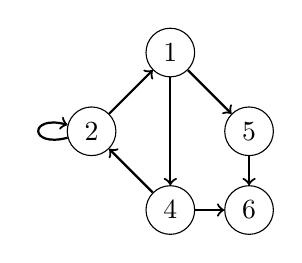
\begin{tikzpicture}[
        every node/.style={draw, minimum size=15pt, circle, text centered},
        ar/.style={->, thick},
        node distance = 22pt,
        invis/.style={draw=none},
    ]

    \node[](1) at (0,1) {1};
    \node[](4) at (0,-1) {4};
    \node[](2) at (-1,0) {2};
    \node[](5) at (1,0) {5};
    \node[](6) at (1,-1) {6};

    \path[ar] 
    (1) edge (5) edge (4)
    (2) edge (1)

    (4) edge (2) edge (6)
    (5) edge (6)
    ;
    \draw[ar, loop left] (2) to (2);
    \end{tikzpicture}
    \captionof*{figure}{Nicht zusammenhängend}
    Kein Pfad von 5 nach 1. (Richtung von (4,6) geändert)
\end{minipage}
\subsubsection{Subgraphen}
Ein Subgraph ist ein Graph, bei dem alle Kanten und Knoten auch in dem übergeordneten Graph liegen.\\
So gilt also $V_s \subseteq V $ und $E_s \subseteq E$.\\
\begin{minipage}[t]{0.5\textwidth}
    \centering
    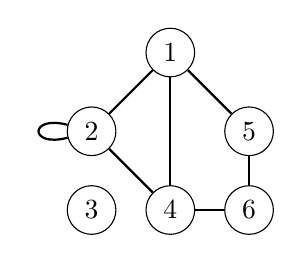
\begin{tikzpicture}[
        every node/.style={draw, minimum size=15pt, circle, text centered},
        ar/.style={-, thick},
        node distance = 22pt,
        invis/.style={draw=none},
    ]

    \node[](1) at (0,1) {1};
    \node[](4) at (0,-1) {4};
    \node[](2) at (-1,0) {2};
    \node[](5) at (1,0) {5};
    \node[](3) at (-1,-1) {3};
    \node[](6) at (1,-1) {6};

    \path[ar] 
    (1) edge (5) edge (4)
    (2) edge (1)

    (4) edge (2)
    (5) edge (6)
    (6) edge (4)
    ;
    \draw[ar, loop left] (2) to (2);
    \end{tikzpicture}
    \captionof*{figure}{Main Graph}
\end{minipage}
\begin{minipage}[t]{0.5\textwidth}
    \centering
    \begin{tikzpicture}[
        every node/.style={draw, minimum size=15pt, circle, text centered},
        ar/.style={-, thick},
        node distance = 22pt,
        invis/.style={draw=none},
    ]

    \node[](1) at (0,1) {1};
    \node[](4) at (0,-1) {4};
    \node[](2) at (-1,0) {2};
    \node[codegray!60](5) at (1,0) {5};
    \node[codegray!60](3) at (-1,-1) {3};
    \node[](6) at (1,-1) {6};

    \path[ar] 
    (1) edge (4)
    (2) edge (1)

    (6) edge (4)
    ;
    \draw[ar, loop left, codegray!60] (2) to (2);
    \draw[ar, codegray!60] (2) to (4);
    \draw[ar, codegray!60] (6) to (5);
    \draw[ar, codegray!60] (5) to (1);
    \end{tikzpicture}
    \captionof*{figure}{Subgraph}
\end{minipage}
\newpage
\subsubsection{Darstellungen}
\textbf{Adjazenzmatrix:}\\
Die Adjazenzliste stellt alle Kanten von einem Knoten zu anderen Knoten in jeder Zeile dar.\\[20pt]
\begin{minipage}[t]{0.5\textwidth}
    \centering
    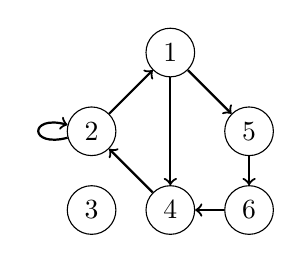
\begin{tikzpicture}[
        every node/.style={draw, minimum size=15pt, circle, text centered},
        ar/.style={->, thick},
        node distance = 22pt,
        invis/.style={draw=none},
    ]

    \node[](1) at (0,1) {1};
    \node[](4) at (0,-1) {4};
    \node[](3) at (-1,-1) {3};
    \node[](2) at (-1,0) {2};
    \node[](5) at (1,0) {5};
    \node[](6) at (1,-1) {6};

    \path[ar] 
    (1) edge (5) edge (4)
    (2) edge (1)

    (4) edge (2)
    (5) edge (6)
    (6) edge (4)
    ;
    \draw[ar, loop left] (2) to (2);
    \end{tikzpicture}
    \captionof*{figure}{Example}
\end{minipage}
\begin{minipage}[t]{0.5\textwidth}
    \centering
    \begin{tikzpicture}[
        array/.style={
            matrix of nodes, nodes={draw ,minimum size =15pt, fill=backcolour, anchor=south},
            row 1/.style={nodes={draw=none, fill=none, color=codegray}},
            row 2/.style={nodes={draw=none, fill=none, color=codegray}},
            column 1/.style={nodes={draw=none, fill=none, color=codegray}},
        },
    ]

    \matrix[array](m){
        to$\rightarrow$   &   &   &   &   &   &   \\
        from $\downarrow$ & 1 & 2 & 3 & 4 & 5 & 6 \\
                        1 & 0 & 0 & 0 & 1 & 1 & 0 \\
                        2 & 1 & 1 & 0 & 0 & 0 & 0 \\
                        3 & 0 & 0 & 0 & 0 & 0 & 0 \\
                        4 & 0 & 1 & 0 & 0 & 0 & 0 \\
                        5 & 0 & 0 & 0 & 0 & 0 & 1 \\
                        6 & 0 & 0 & 0 & 1 & 0 & 0 \\
    };
    \end{tikzpicture}
\end{minipage}\\[20pt]
Für ungerichtete Graphen ist die Adjazenzmatrix spiegelsymmetrisch zur Hauptdiagonalen.\\
Die Adjazenzmatrix hat die Eigenschaft, dass der Eintrag $a_{i,j}^{(m)}$ ($i$-te Zeile, $j$-te Spalte der $m$-ten ($A^m$) Potenz der Matrix $A$) die Anzahl der Wege von Knoten $i$ zum Knoten $j$ mit genau $m$ Kanten besitzt.

\textbf{Adjazenzliste:}\\
Die Adjazenliste stellt die Kanten von einem Knoten zu anderen Knoten als Array mit verketteten Listen dar.\\[20pt]
\begin{minipage}[t]{0.5\textwidth}
    \centering
    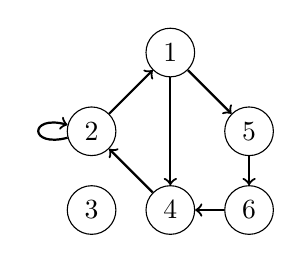
\begin{tikzpicture}[
        every node/.style={draw, minimum size=15pt, circle, text centered},
        ar/.style={->, thick},
        node distance = 22pt,
        invis/.style={draw=none},
    ]

    \node[](1) at (0,1) {1};
    \node[](4) at (0,-1) {4};
    \node[](3) at (-1,-1) {3};
    \node[](2) at (-1,0) {2};
    \node[](5) at (1,0) {5};
    \node[](6) at (1,-1) {6};

    \path[ar] 
    (1) edge (5) edge (4)
    (2) edge (1)

    (4) edge (2)
    (5) edge (6)
    (6) edge (4)
    ;
    \draw[ar, loop left] (2) to (2);
    \end{tikzpicture}
    \captionof*{figure}{Example}
\end{minipage}
\begin{minipage}[t]{0.5\textwidth}
    \centering
    \begin{tikzpicture}[
        invis/.style={draw=none, minimum size = 15pt, fill=none, color=codegray, anchor=south},
        table/.style={minimum width=25pt, minimum height=15pt, draw, rectangle, anchor=south},
        linked/.style={minimum width = 20pt, minimum height = 12.5pt, draw, rectangle, rounded corners},
        ar/.style={<->, thick},
        node distance = 20pt,
    ]

    \node[invis](1i){1};
    \node[invis, below = 0 of 1i](2i){2};
    \node[invis, below = 0 of 2i](3i){3};
    \node[invis, below = 0 of 3i](4i){4};
    \node[invis, below = 0 of 4i](5i){5};
    \node[invis, below = 0 of 5i](6i){6};


    \node[table, right = 0 of 1i](1-1){4};
    \node[table, right = of 1-1](1-2){5};

    \node[table, below = 0 of 1-1](2-1){1};
    \node[table, right = of 2-1](2-2){2};

    \node[table, below = 0 of 2-1](3-1){};

    \node[table, below = 0 of 3-1](4-1){2};

    \node[table, below = 0 of 4-1](5-1){6};

    \node[table, below = 0 of 5-1](6-1){4};

    \draw[ar] (1-1) to (1-2);
    \draw[ar] (2-1) to (2-2);

    \end{tikzpicture}
\end{minipage}

\newpage
\subsection{Breadth-First Search (BFS)}
Der Breadth-First Search Algorithmus funktioniert nach dem Prinzip, dass von dem Startpunkt aus erst alle direkten Nachbarn besucht werden. Anschließend werden alle Nachbarn der direkten Nachbarn besucht und so weiter.
\begin{minipage}[t]{0.33\textwidth}
    \centering
    \begin{tikzpicture}[
        every node/.style={draw, minimum size=15pt, circle, text centered},
        ar/.style={->, thick},
        node distance = 22pt,
        invis/.style={draw=none},
        queued/.style={fill=codegray!50},
        finished/.style={fill=codegray},
    ]

    \node[queued](1) at (0,1) {1};
    \node[](4) at (0,-1) {4};
    \node[](2) at (-1,0) {2};
    \node[](5) at (1,0) {5};
    \node[](3) at (-1,-1) {3};
    \node[](6) at (1,-1) {6};

    \node[invis, above =-15pt of 1] {\small(0/NIL)}; 

    \path[ar] 
    (1) edge (5) edge (4)
    (2) edge (1)

    (4) edge (2) edge (5)
    (5) edge (6)
    (6) edge (4)
    ;
    \draw[ar, loop left] (2) to (2);
    \end{tikzpicture}\\
    Q = (1)
\end{minipage}
\begin{minipage}[t]{0.33\textwidth}
    \centering
    \begin{tikzpicture}[
        every node/.style={draw, minimum size=15pt, circle, text centered},
        ar/.style={->, thick},
        node distance = 22pt,
        invis/.style={draw=none},
        queued/.style={fill=codegray!50},
        finished/.style={fill=codegray},
    ]

    \node[finished](1) at (0,1) {1};
    \node[queued](4) at (0,-1) {4};
    \node[](2) at (-1,0) {2};
    \node[queued](5) at (1,0) {5};
    \node[](3) at (-1,-1) {3};
    \node[](6) at (1,-1) {6};

    \node[invis, below =-10pt of 4] {\small(1/1)}; 
    \node[invis, above =-10pt of 5] {\small(1/1)}; 

    \path[ar] 
    (1) edge (5) edge (4)
    (2) edge (1)

    (4) edge (2) edge (5)
    (5) edge (6)
    (6) edge (4)
    ;
    \draw[ar, loop left] (2) to (2);
    \end{tikzpicture}\\
    Q = (4,5)
\end{minipage}
\begin{minipage}[t]{0.33\textwidth}
    \centering
    \begin{tikzpicture}[
        every node/.style={draw, minimum size=15pt, circle, text centered},
        ar/.style={->, thick},
        node distance = 22pt,
        invis/.style={draw=none},
        queued/.style={fill=codegray!50},
        finished/.style={fill=codegray},
    ]

    \node[finished](1) at (0,1) {1};
    \node[finished](4) at (0,-1) {4};
    \node[queued](2) at (-1,0) {2};
    \node[queued](5) at (1,0) {5};
    \node[](3) at (-1,-1) {3};
    \node[](6) at (1,-1) {6};

    \node[invis, above =-10pt of 2] {\small(2/4)}; 
    \node[invis, above =-10pt of 5] {\small(1/1)}; 

    \path[ar] 
    (1) edge (5) edge (4)
    (2) edge (1)

    (4) edge (2) edge (5)
    (5) edge (6)
    (6) edge (4)
    ;
    \draw[ar, loop left] (2) to (2);
    \end{tikzpicture}\\
    Q = (5,2)
\end{minipage}\\[20pt]
\begin{minipage}[t]{0.33\textwidth}
    \centering
    \begin{tikzpicture}[
        every node/.style={draw, minimum size=15pt, circle, text centered},
        ar/.style={->, thick},
        node distance = 22pt,
        invis/.style={draw=none},
        queued/.style={fill=codegray!50},
        finished/.style={fill=codegray},
    ]

    \node[finished](1) at (0,1) {1};
    \node[finished](4) at (0,-1) {4};
    \node[queued](2) at (-1,0) {2};
    \node[finished](5) at (1,0) {5};
    \node[](3) at (-1,-1) {3};
    \node[queued](6) at (1,-1) {6};

    \node[invis, above =-10pt of 2] {\small(2/4)};
    \node[invis, below =-10pt of 6] {\small(2/5)}; 

    \path[ar] 
    (1) edge (5) edge (4)
    (2) edge (1)

    (4) edge (2) edge (5)
    (5) edge (6)
    (6) edge (4)
    ;
    \draw[ar, loop left] (2) to (2);
    \end{tikzpicture}\\
    Q = (2,6)
\end{minipage}
\begin{minipage}[t]{0.33\textwidth}
    \centering
    \begin{tikzpicture}[
        every node/.style={draw, minimum size=15pt, circle, text centered},
        ar/.style={->, thick},
        node distance = 22pt,
        invis/.style={draw=none},
        queued/.style={fill=codegray!50},
        finished/.style={fill=codegray},
    ]

    \node[finished](1) at (0,1) {1};
    \node[finished](4) at (0,-1) {4};
    \node[finished](2) at (-1,0) {2};
    \node[finished](5) at (1,0) {5};
    \node[](3) at (-1,-1) {3};
    \node[queued](6) at (1,-1) {6};

    \node[invis, below =-10pt of 6] {\small(2/5)}; 

    \path[ar] 
    (1) edge (5) edge (4)
    (2) edge (1)

    (4) edge (2) edge (5)
    (5) edge (6)
    (6) edge (4)
    ;
    \draw[ar, loop left] (2) to (2);
    \end{tikzpicture}\\
    Q = (6)
\end{minipage}
\begin{minipage}[t]{0.33\textwidth}
    \centering
    \begin{tikzpicture}[
        every node/.style={draw, minimum size=15pt, circle, text centered},
        ar/.style={->, thick},
        node distance = 22pt,
        invis/.style={draw=none},
        queued/.style={fill=codegray!50},
        finished/.style={fill=codegray},
    ]

    \node[finished](1) at (0,1) {1};
    \node[finished](4) at (0,-1) {4};
    \node[finished](2) at (-1,0) {2};
    \node[finished](5) at (1,0) {5};
    \node[](3) at (-1,-1) {3};
    \node[finished](6) at (1,-1) {6};

    \node[invis,rectangle, below =0pt of 3] {\small($+\infty$/NIL)}; 

    \path[ar] 
    (1) edge (5) edge (4)
    (2) edge (1)

    (4) edge (2) edge (5)
    (5) edge (6)
    (6) edge (4)
    ;
    \draw[ar, loop left] (2) to (2);
    \end{tikzpicture}\\
    Q = ()
\end{minipage}


Nach dem Ausführen von BFS kann man durch die jetzt gegebenen Vorgängern einen Subgraphen ableiten.\\
\begin{minipage}[t]{0.5\textwidth}
    \centering
    \begin{tikzpicture}[
        every node/.style={draw, minimum size=15pt, circle, text centered},
        ar/.style={->, thick},
        node distance = 22pt,
        invis/.style={draw=none, rectangle},
        queued/.style={fill=codegray!50},
        finished/.style={fill=codegray},
    ]

    \node[finished](1) at (0,1) {1};
    \node[finished](4) at (0,-1) {4};
    \node[finished](2) at (-1,0) {2};
    \node[finished](5) at (1,0) {5};
    \node[](3) at (-1,-1) {3};
    \node[finished](6) at (1,-1) {6};

    \node[invis, below =9.5pt of 3.west] {\small($+\infty$/NIL)}; 
    \node[invis, above =0 of 1] {\small(0/NIL)};
    \node[invis, above =0 of 5] {\small(1/1)};
    \node[invis, below =0 of 4] {\small(1/1)};
    \node[invis, below =0 of 6] {\small(2/5)};
    \node[invis, above =0 of 2] {\small(2/4)};

    \path[ar] 
    (1) edge (5) edge (4)
    (2) edge (1)

    (4) edge (2) edge (5)
    (5) edge (6)
    (6) edge (4)
    ;
    \draw[ar, loop left] (2) to (2);
    \end{tikzpicture}
    \captionof*{figure}{Graph nach BFS}
\end{minipage}
\begin{minipage}[t]{0.5\textwidth}
    \centering
    \begin{tikzpicture}[
        every node/.style={draw, minimum size=15pt, circle, text centered},
        ar/.style={->, thick},
        node distance = 20pt,
    ]
    \node[](1){1};
    \node[below left =of 1](4){4};
    \node[below right =of 1](5){5};
    \node[below =15pt of 4](2){2};
    \node[below =15pt of 5](6){6};

    \path[ar]
    (1) edge (4) edge (5)
    (4) edge (2)
    (5) edge (6)
    ;
    \end{tikzpicture}\\
    \captionof*{figure}{Abgeleiteter Subgraph}
\end{minipage}\\[20pt]
Der Subgraph ist durch $V_{pred}^s = \{v \in V | v.pred \not= $NIL$\} \cup \{s\}$ und $E_{pred}^s = \{(v.pred, v) | v \in V_{pred}^s - \{s\}\}$ gegeben. D.h. bedeutet, dass der Subgraph alle von $s$ erreichbaren Knoten enthält und für jeden Knoten im Subgraph genau ein Pfad von $s$, der auch automatisch der kürzeste Pfad von $s$ zu $v$ ist, existiert.
\includepdf[pages={20,29}, pagecommand={},nup=1x2, frame=true, scale=0.9]{./VL Folien/06GraphAlgorithms.pdf}
\subsection{Depth-First Search (DFS)}

\includepdf[pages={35,63}, pagecommand={},nup=1x2, frame=true, scale=0.9]{./VL Folien/06GraphAlgorithms.pdf}
\subsection{Strongly Connected Components (SCC)}

\newpage
\subsection{Minimale Spannbäume (MST)}
\subsubsection{Kruskals Algorithmus}
\subsubsection{Prims Algorithmus}

\newpage
\subsection{Kürzesten Pfade}
\subsubsection{Bellman-Ford Algorithmus}
\subsubsection{Dags Algorithmus}
\subsubsection{Dijkstra Algorithmus}

\newpage
\subsection{Maximaler Fluss}
\subsubsection{Ford-Fulkerson Algorithmus}
\end{document}